\documentclass[11pt]{article}
\setlength{\parindent}{0pt}
\usepackage[a4paper,margin=1in]{geometry}
\usepackage{amsmath,amssymb}
\usepackage[T1]{fontenc}
\usepackage{tikz}
\usetikzlibrary{matrix,fit,backgrounds,calc}
\usepackage{comment}
\usepackage{amsmath}
\usepackage{bm}

\newcommand{\quaternion}[1]{\bm{\mathrm{#1}}}

\title{Quaternion Multiplication: Scalar, Vector, Dot, and Cross Products}
\author{}
\date{}

\begin{document}
\maketitle


\section{Denoting quaternions and vectors.}

In this article, we will denote quaternions using uppercase letters, while vectors will be denoted using either lowercase
or uppercase letters which have been adorned with a right pointing arrow above them. Examples of how vectors will be denoted are
shown immediately below;

\begin{equation*}
\vec{v} \quad \vec{V} \quad \vec{q} \quad \vec{Q}
\end{equation*}


\newpage
\section{Quaternions.}

Quaternions are very similar to complex numbers. However, whereas complex numbers are comprised of one real component and one
imaginary component, quaternions are comprised of one real component and three imaginary components, for a grand total of four
components all up. Since quaternions are comprised of multiple imaginary components, they are categorised as
``hypercomplex numbers'' and because they are comprised of four components in total, this explains why they are
called ``quaternions''; since ``quat'' means of or relating to four parts. \\

A quaternion is often denoted using one of the following forms;

\begin{align*}
Q & = w   + \quaternion{i} x   + \quaternion{i} y   + \quaternion{k} z  \\
Q & = a   + \quaternion{i} b   + \quaternion{j} c   + \quaternion{k} d  \\
Q & = Q_0 + \quaternion{i} Q_1 + \quaternion{j} Q_2 + \quaternion{k} Q_3
\end{align*}
\vspace{0.0\baselineskip}

The first component, or the real component of the quaternion, i.e. \(w\), \(a\), or \(Q_0\) in the previous examples,
is often referred to as the scalar part of the quaternion, while the remaining three components are collectively
referred to as the vector part of the quaternion.

\begin{equation*}
Q = \underbrace{w}_{\text{scalar}} + \underbrace{\quaternion{i}x + \quaternion{j}y + \quaternion{k}z}_{\text{vector}}
\end{equation*}

If we were to denote the vector component of the quaternion \(Q\) as \(\vec{Q}\), then we could rewrite the three example
quaternions from above as follows;

\begin{align*}
    Q & = w + \vec{Q}  \\
    Q & = a + \vec{Q}  \\
    Q & = Q_0 + \vec{Q}
\end{align*}
\vspace{0.0\baselineskip}

where;

\begin{align*}
    \vec{Q} &= (\quaternion{i}x, \quaternion{j}y, \quaternion{k}z) \; \text{or}  \\
            &= (\quaternion{i}b, \quaternion{j}c, \quaternion{k}d) \; \text{or}  \\
            &= (\quaternion{i}Q_{1}, \quaternion{j}Q_{2}, \quaternion{k}Q_{3})
\end{align*}


\subsection{Pure quaternions.}

A pure quaternion -- also referred to sometimes as a purely imaginary quaternion, is one whose real or scalar component
is equal to zero. That is, if we have;

\begin{equation*}
    Q = Q_0 + Q_1 + Q_2 + Q_3 \; \; \; \; \; \; \mid \; \; Q_0 = 0
\end{equation*}
\vspace{0.0\baselineskip}

then;

\begin{align*}
    Q & = 0 + Q_1 + Q_2 + Q_3  \\
      & = \vec{Q}
\end{align*}
\vspace{0.0\baselineskip}
as oppo

\subsection{Unit quaternions.}

A unit quaternion -- not to be confused with a quaternion unit such as \(1\), \(\quaternion{i}\), \(\quaternion{j}\), or
\(\quaternion{k}\), is a quaternion whose length or magnitude is equal to one. For example, the following quaternions
are all unit quaternions, because they all have a length or magnitude of one;

\begin{align*}
    Q1 & = 1  \\
    Q2 & = 0.5 + \quaternion{i}0.5 + \quaternion{j}0.5 + \quaternion{k}0.5  \\
    Q3 & = 0.707 + \quaternion{i}0.707  \\
    Q4 & = \quaternion{i}0.577 + \quaternion{j}0.577 + \quaternion{k}0.577
\end{align*}
\vspace{0.0\baselineskip}

To illustrate, first consider the quaternion \(Q2\).

\begin{align*}
    \lVert Q2 \rVert & = \sqrt{0.5^2 + 0.5^2 + 0.5^2 + 0.5^2}  \\
                     & = \sqrt{0.25 + 0.25 + 0.25 + 0.25}  \\
                     & = \sqrt{1}  \\
                     & = 1
\end{align*}
\vspace{0.0\baselineskip}

Next consider the quaternion \(Q4\).

\begin{align*}
    \lVert Q4 \rVert & = \sqrt{0.577^2 + 0.577^2 + 0.577^2}  \\
                     & = \sqrt{0.333 + 0.333 + 0.333}  \\
                     & = \sqrt{1}  \\
                     & = 1
\end{align*}
\vspace{0.0\baselineskip}

It might be worth noting - but then again it might not, that when taken altogether, all of the unit quaternions form the
surface of a 4-dimensional hypersphere. I mention that this might not be worth noting, because the concept of a
4-dimensional hypersphere seems almost incomprehensible to some people nd they would rather not have to think about it!


\subsection{Quaternion units and rules.}

Let's recall our three example quaternions from earlier, that is;

\begin{align*}
Q & = w   + \quaternion{i} x   + \quaternion{i} y   + \quaternion{k} z  \\
Q & = a   + \quaternion{i} b   + \quaternion{j} c   + \quaternion{k} d  \\
Q & = Q_0 + \quaternion{i} Q_1 + \quaternion{j} Q_2 + \quaternion{k} Q_3
\end{align*}
\vspace{0.0\baselineskip}

In these three examples, \(1\), \(\quaternion{i}\), \(\quaternion{j}\), and \(\quaternion{k}\) are all known as
quaternion units, even though it is only \(\quaternion{i}\), \(\quaternion{j}\), and \(\quaternion{k}\) which are
explicitly depicted in the three previous definitions of \(Q\). \\

When it comes to multiplying these units with themselves and each other, they satisfy the following rules;

\begin{equation*}
\quaternion{i}^2=\quaternion{j}^2=\quaternion{k}^2=\quaternion{ijk}=-1
\end{equation*}
\vspace{0.0\baselineskip}

From this, the following additional multiplication rules can also be derived;

\begin{equation*}
\quaternion{ij}=\quaternion{k},\quad \quaternion{jk}=\quaternion{i},\quad \quaternion{ki}=\quaternion{j},
\end{equation*}

as well as;

\begin{equation*}
\quaternion{ji}=-\quaternion{k}, \quad \quaternion{kj}=-\quaternion{i},\quad \quaternion{ik}=-\quaternion{j}
\end{equation*}


\newpage
\section{Multiplying two quaternions together.}

Now consider another quaternion, which we will name \(P\).

\begin{equation*}
P = P_0 + \quaternion{i}P_1 + \quaternion{j}P_2 + \quaternion{k}P_3
\end{equation*}
\vspace{0.0\baselineskip}

Just like we did for quaternion \(Q\), we can also define this quaternion in terms of its scalar and vector components;

\begin{equation*}
P = P_0 + \vec{P}
\end{equation*}
\vspace{0.0\baselineskip}

We can multiply this quaternion with the earlier quaternion \(Q\) as follows;

\begin{equation*}
PQ = (P_0 + \quaternion{i}P_1 + \quaternion{j}P_2 + \quaternion{k}P_3)(Q_0 + \quaternion{i}Q_1 + \quaternion{j}Q_2 + \quaternion{k}Q_3)
\end{equation*}
\vspace{0.0\baselineskip}

Expanding this out gives the following;

\begin{align*}
PQ = {}& \;   P_0(Q_0 + iQ_1 + jQ_2 + kQ_3) \; + \\
       &     \quaternion{i}P_1(Q_0 + \quaternion{i}Q_1 + \quaternion{j}Q_2 + \quaternion{k}Q_3) \; + \\
       &     \quaternion{j}P_2(Q_0 + \quaternion{i}Q_1 + \quaternion{j}Q_2 + \quaternion{k}Q_3) \; + \\
       & \!  \quaternion{k}P_3(Q_0 + \quaternion{i}Q_1 + \quaternion{j}Q_2 + \quaternion{k}Q_3)
\end{align*}

Expanding even further gives;

\begin{align*}
PQ = {}& \;                P_0Q_0      + \;\, \quaternion{i}P_0Q_1 \,  + \quaternion{j}P_0Q_2 +   \quaternion{k}P_0Q_3 \;  + \\
       &     \quaternion{i}P_1Q_0      + \,   \quaternion{i}^2P_1Q_1   + \quaternion{ij}P_1Q_2 +  \quaternion{ik}P_1Q_3 \; + \\
       &     \quaternion{j}P_2Q_0 \,\! + \,\! \quaternion{ji}P_2Q_1 \, + \quaternion{j}^2P_2Q_2 + \quaternion{jk}P_2Q_3 \; + \\
       & \!  \quaternion{k}P_3Q_0      +      \quaternion{ki}P_3Q_1    + \quaternion{kj}P_3Q_2 +  \quaternion{k}^2P_3Q_3
\end{align*}

Applying the multiplication rules;

\begin{align*}
PQ = {}& \;                P_0Q_0 + \quaternion{i}P_0Q_1 + \quaternion{j}P_0Q_2 + \quaternion{k}P_0Q_3 \; + \\
       &     \quaternion{i}P_1Q_0 - P_1Q_1               + \quaternion{k}P_1Q_2 - \quaternion{j}P_1Q_3 \; + \\
       & \!  \quaternion{j}P_2Q_0 - \quaternion{k}P_2Q_1 - P_2Q_2               + \quaternion{i}P_2Q_3 \; + \\
       & \!  \quaternion{k}P_3Q_0 + \quaternion{j}P_3Q_1 - \quaternion{i}P_3Q_2 - P_3Q_3
\end{align*}

Collecting the scalar, \(i\), \(j\), and \(k\) terms gives
\begin{align*}
PQ = {} &          (P_0Q_0 - P_1Q_1 - P_2Q_2 - P_3Q_3) + \\
        & \quaternion{i} (P_0Q_1 + P_1Q_0 + P_2Q_3 - P_3Q_2) + \\
        & \quaternion{j} (P_0Q_2 - P_1Q_3 + P_2Q_0 + P_3Q_1) + \\
        & \quaternion{k} (P_0Q_3 + P_1Q_2 - P_2Q_1 + P_3Q_0)
\end{align*}


\newpage
\section{Analysing the final result.}

Before we proceed any further, let us first rewrite the final result from the previous section. However this time, as
part of the process of rewriting the final result, let us also highlight those terms which have certain particular
features in common with other terms. As you may have already noticed from the final result in the previous section --
or should hopefully notice in a moment, some of the terms share features with multiple other terms, while others share
features with only one other term.\\

Rewriting and highlighting the final result yields the following;

\[
    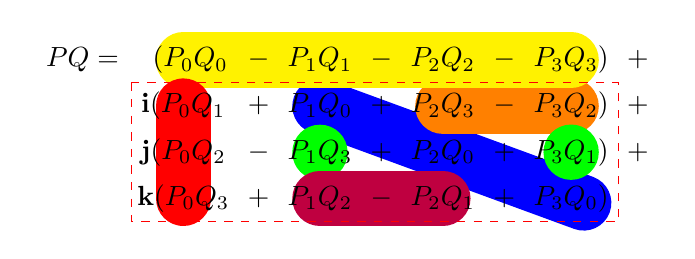
\begin{tikzpicture}
        \matrix (m)
        [
            matrix of math nodes,
            row sep=0pt,
            column sep=0pt
        ]
        {
            PQ = & |[name=m-1-1]| \, (P_0Q_0 \!\! & - & |[name=m-1-2]|P_1Q_1 & - & |[name=m-1-3]|P_2Q_2 & - & |[name=m-1-4]|P_3Q_3) & + &  \\
                 & |[name=m-2-1]|\quaternion{i}(P_0Q_1         & + & |[name=m-2-2]|P_1Q_0 & + & |[name=m-2-3]|P_2Q_3 & - & |[name=m-2-4]|P_3Q_2) & + &  \\
                 & |[name=m-3-1]|\quaternion{j}(P_0Q_2         & - & |[name=m-3-2]|P_1Q_3 & + & |[name=m-3-3]|P_2Q_0 & + & |[name=m-3-4]|P_3Q_1) & + & \\
                 & |[name=m-4-1]|\quaternion{k}(P_0Q_3         & + & |[name=m-4-2]|P_1Q_2 & - & |[name=m-4-3]|P_2Q_1 & + & |[name=m-4-4]|P_3Q_0)  \\
        };

        \draw[dashed, red, thin]
            (m-2-1.north west) rectangle (m-4-4.south east);

        \begin{scope}[on background layer]
        \draw[blue, line width=20pt, opacity=1.00, line cap=round]
           ($(m-2-2.center)+(0,0)$) -- ($(m-2-2.center)!1.05!(m-4-4.center)$);
        \end{scope}

        \begin{scope}[on background layer]Straight
        \draw[orange, line width=20pt, opacity=1.00, line cap=round]
            ($(m-2-3.center)+(0,0)$) -- ($(m-2-4.center)$);
        \end{scope}

        \begin{scope}[on background layer]
        \draw[green, line width=20pt, opacity=1.00, line cap=round]
            ($(m-3-2.center)+(0,0)$) -- ($(m-3-2.center)$);
        \end{scope}

        \begin{scope}[on background layer]
        \draw[purple, line width=20pt, opacity=1.00, line cap=round]
            ($(m-4-2.center)+(0,0)$) -- ($(m-4-3.center)$);
        \end{scope}

        \begin{scope}[on background layer]
        \draw[green, line width=20pt, opacity=1.00, line cap=round]
            ($(m-3-4.center)+(0,0)$) -- ($(m-3-4.center)$);
        \end{scope}

                \begin{scope}[on background layer]
        \draw[yellow, line width=20pt, opacity=1.00, line cap=round]
            ($(m-1-1.center)+(0,0)$) -- ($(m-1-4.center)$);
        \end{scope}

        \begin{scope}[on background layer]
        \draw[red, line width=20pt, opacity=1.00, line cap=round]
            ($(m-2-1.center)+(0,0)$) -- ($(m-4-1.center)$);
        \end{scope}

    \end{tikzpicture}
\]

Note that the final result is composed of sixteen different terms and that;

\begin{itemize}
    \item four of these terms make use of the quaternion unit \(1\), and
    \item the other twelve of these terms make use of one of the three imaginary quaternion units, i.e. \(\quaternion{i}\),
          \(\quaternion{j}\), or
          \(\quaternion{k}\).
\end{itemize}

The four terms which make use of the quaternion unit \(1\) are highlighted in yellow and when taken together, they act
as a scalar component within the final result.\\

The other twelve terms which make up the final result are surrounded by a thin dashed red line, and when taken together,
they act as a vector component within the final result.


\subsection{The scalar component of the final result.}

As we said only a moment ago, the four terms which make use of the quaternion unit 1 are highlighted in yellow and when
taken together, they act as a scalar component within the final result. Upon inspection of these four terms, you should
be able to see that this scalar component can be defined as follows;

\vspace{0.25\baselineskip}

\begin{equation*}
    \text{Scalar component}(PQ) = P_{0}Q_{0} - \vec{P} \cdot \vec{Q}
\end{equation*}
\vspace{0.0\baselineskip}

where \(\vec{P} \cdot \vec{Q}\) denotes the dot, scalar, or inner product between the two vectors \(\vec{P}\) and
\(\vec{Q}\).


\subsection{The vector component of the final result.}

Once again, as we said only a moment ago, the other twelve terms which make up the final result are surrounded by a thin
dashed red line, and when taken together, they act as a vector component within the final result. \\

\textbullet \; The term : \(P_{0}\vec{Q}\) \\

Within these twelve terms, we can see straight away that the three terms which have been highlighted in red can be
defined as;

\begin{equation*}
    P_{0}\vec{Q}
\end{equation*}
\vspace{0.0\baselineskip}

where;

\begin{equation*}
    \vec{Q} = \quaternion{i}Q_1 + \quaternion{j}Q_2 + \quaternion{k}Q_3
\end{equation*}
\vspace{0.0\baselineskip}

\textbullet \; The term : \(\vec{P}Q_{0}\) \\

Similarly, we can see that the three terms which have been highlighted in blue can be defined as;

\begin{equation*}
    \vec{P}Q_{0}
\end{equation*}

where;

\begin{equation*}
    \vec{P} = \quaternion{i}P_1 + \quaternion{j}P_2 + \quaternion{k}P_3
\end{equation*}
\vspace{0.0\baselineskip}

\textbullet \; The term : \(\vec{P} \times \vec{Q}\) \\

Now all that's left, are the terms which are highlighted in orange, green, and purple. If you are familiar with
determinants, you might notice that we can generate these exact same terms using determinants and an appropriately
populated \(3 \times 3\) matrix. In order to do this, we would need a \(3 \times 3\) matrix which is populate as
follows;

\begin{equation*}
    \begin{vmatrix}
        \quaternion{i} & \quaternion{j} & \quaternion{k} \\
        P_1      & P_2      & P_3      \\
        Q_1      & Q_2      & Q_3
    \end{vmatrix}
\end{equation*}
\vspace{0.0\baselineskip}

Evaluating this determinant gives us what is known as the cross product of \(\vec{P}\) and \(\vec{Q}\), and which is
denoted mathematically as;

\begin{equation*}
    \vec{P} \times \vec{Q}
\end{equation*}
\vspace{0.0\baselineskip}

As a point of interest, note that the cross product doesn't contain any real terms. That is, it doesn't contain either
\(P_0\) or \(Q_0\). Keep this in mind, as we will return to this fact again later. \\

We won't discuss the cross product any further here, however we will return to it soon. \\

\textbullet \; Bringing these three terms together. \\

We have now accounted for all twelve of the terms which comprise the vector component of the final result. If we sum
together all three of the terms which we just derived, then we end up with following definition for our vector component.

\begin{equation*}
    \text{Vector component}(PQ) = P_0\vec{Q} + Q_0\vec{P} + (\vec{P}\times\vec{Q})
\end{equation*}

where;

\begin{itemize}
    \item \(P_0\vec{Q}\) corresponds to all of the elements in the final result which are highlighted in red.
    \item \(Q_0\vec{P}\) corresponds to all of the elements in the final result which are highlighted in blue.
    \item \(\vec{P}\times\vec{Q}\) corresponds to all of the elements in the final result which are highlighted in
                              orange, green, and purple.
\end{itemize}

From this, we can see that the vector component of the final result is comprised of two scalar products and one cross
product.


\newpage
\section{Adding the scalar and vector parts together.}

If we bring together our definitions for the scalar part and the vector part of the final result, then we will get
the following result for our quaternion multiplication \(PQ\);

\begin{align*}
PQ &= \text{Scalar component}(PQ) + \text{Vector component}(PQ)  \\
   &= \bigr(P_{0}Q_{0} - \vec{P} \cdot \vec{Q}\bigr) \, + \, \bigr(P_0\vec{Q} + Q_0\vec{P} + (\vec{P}\times\vec{Q})\bigr)
\end{align*}


\subsection{What if \(P\) and \(Q\) were pure quaternions?}

If \(P\) and \(Q\) were pure quaternions, then \(P_0\) and \(Q_0\) would boths be equal to zero. In that case we would
get;

\begin{align*}
PQ & = \bigl(P_{0}Q_{0} - \vec{P} \cdot \vec{Q}\bigr) \, + \, \bigr(P_0\vec{Q} + Q_0\vec{P} + (\vec{P}\times\vec{Q})\bigr)  \\
   & = \bigl((0 \times 0) - \vec{P} \cdot \vec{Q}\bigr) \, + \, \bigr((0 \times \vec{Q}) + (0 \times \vec{P}) + (\vec{P} \times \vec{Q})\bigr)  \\
   & = \bigl(0 - \vec{P} \cdot \vec{Q}\bigr) \, + \, \bigr(0 + 0 + (\vec{P}\times\vec{Q})\bigr)  \\
   & = -(\vec{P} \cdot \vec{Q}) \, + \, (\vec{P} \times \vec{Q})
\end{align*}

Notice that three of the terms have disappeared and we are now left with jsut two terms -- the dot product between \(P\)
and \(Q\), and the cross product between \(P\) and \(Q\).

\newpage
\section{The cross product : \((\vec{P}\times\vec{Q})\)}

Earlier, we stated that the cross product components of \(\vec{P}\times\vec{Q}\) can be calculated by evaluating the
determinant of the following matrix, which we will arbitrarily call \(A\) here.

\begin{equation*}
    A = \begin{vmatrix}
        \quaternion{i} & \quaternion{j} & \quaternion{k}  \\
        P_1      & P_2      & P_3       \\
        Q_1      & Q_2      & Q_3
        \end{vmatrix}
\end{equation*}
\vspace{0.0\baselineskip}

Calculating the determinant of this matrix proceeds as follows;

\begin{equation*}
    \det{(A)} = \quaternion{i}
    \begin{vmatrix}
        P_2        & P_3  \\
        Q_2        & Q_3
    \end{vmatrix}
    -
    \quaternion{j}
    \begin{vmatrix}
        P_1        & P_3  \\
        Q_1        & Q_3
    \end{vmatrix}
    +
    \quaternion{k}
    \begin{vmatrix}
        P_1        & P_2  \\
        Q_1        & Q_2
    \end{vmatrix}
\end{equation*}
\vspace{0.0\baselineskip}

Expanding this out gives the following;

\begin{equation*}
    \det{(A)} = \quaternion{i}(P_2Q_3 - P_3Q_2) - \quaternion{j}(P_1Q_3 - P_3Q_1) + \quaternion{k}(P_1Q_2 - P_2Q_1)
\end{equation*}
\vspace{0.0\baselineskip}

Which then simplifies one step further to become;

\begin{equation*}
    \det{(A)} = \quaternion{i}(P_2Q_3 - P_3Q_2) + \quaternion{j}(P_3Q_1 - P_1Q_3) + \quaternion{k}(P_1Q_2 - P_2Q_1)
\end{equation*}


\subsection{A very brief history of how the cross product came about.}

If you have ever studied the cross product before and wondered why it is defined in the manner in which it is -- this is
it. That is, it came about in large part thanks to William Rowan Hamilton and his development of quaternions and
quaternion multiplication along with the rules governing it, in the 1840s. We use the expression
``in large part'', because it is widely believed that Hamilton never actually used the term ``cross product'' for that
part of the result which we looked at earlier. Instead, it is reported that he just considered the result of a
quaternion multiplication to be composed of a scalar part and a vector part. Later in the 1800s, Oliver Heaviside and
Josiah Willard Gibbs built on Hamilton's work with quaternions to formalise the mathematical concept of vector. It is
from their work, that the idea of the cross product came about and was subsequently named as such. \\

However, other figures were also involved in work which was relevant to the development of the cross product. In the
1770s, Joseph Louis Lagrange developed formulas which are algebraically equivalent to the cross product. Around the same
time that Hamilton developed the quaternion, Hermann Grassmann also undertook work which helped contribute to the
cross product as we know it today.


\subsection{What does the cross product actually mean?}

We have talked somewhat at length about the cross


\subsection*{3. Identify the dot and cross products}

The ordinary three-dimensional dot product is
\[
\mathbf P\cdot\mathbf Q
=P_1Q_1+P_2Q_2+P_3Q_3.
\]

Therefore,
\[
\operatorname{Sc}(PQ)
=P_0Q_0-\mathbf P\cdot\mathbf Q.
\]

The ordinary three-dimensional cross product is
\[
\mathbf P\times\mathbf Q
=
\begin{pmatrix}
P_2Q_3-P_3Q_2\\
P_3Q_1-P_1Q_3\\
P_1Q_2-P_2Q_1
\end{pmatrix}.
\]

The vector part can consequently be written as
\[
\operatorname{Vec}(PQ)
=P_0\mathbf Q+Q_0\mathbf P+\mathbf P\times\mathbf Q.
\]

Thus the complete quaternion product is
\[
\boxed{
PQ=
\left(P_0Q_0-\mathbf P\cdot\mathbf Q\right)
+
\left(P_0\mathbf Q+Q_0\mathbf P+\mathbf P\times\mathbf Q\right)
}.
\]

Here the first parentheses contain the scalar part, and the second parentheses contain the vector part.

\section*{4. Why the cross product appears}

For example, the terms contributing to the \(i\)-component include
\[
(jP_2)(kQ_3)=iP_2Q_3,
\]
whereas
\[
(kP_3)(jQ_2)=-iP_3Q_2.
\]

Together they give
\[
i(P_2Q_3-P_3Q_2),
\]
which is the \(i\)-component of
\(\mathbf P\times\mathbf Q\).

The \(j\)- and \(k\)-components arise in the same way:
\[
j(P_3Q_1-P_1Q_3),
\]
\[
k(P_1Q_2-P_2Q_1).
\]

The cross product therefore emerges from the antisymmetric part of quaternion multiplication.

\end{document}